\section{Zarys problemu}

Po przeanalizowaniu wydajności Raspberry Pi, postanowiliśmy zredukować zakres odpowiedzialności płytki, aby będąc w kosmosie robiła zdjęcia powierzchni Ziemi i zapisywała je na karcie pamięci.
Zdjęcia mają następnie trafić do nas, w celu dalszej analizy.
Zależy nam na dużej ilości danych, ale ponieważ zasady konkursu (oraz, rzecz jasna, pojemność karty pamięci płytki Raspberry Pi) narzucają na nas ograniczenia względem zurzytej przestrzeni dyskowej,
chcemy przechowywać zdjęcia o jak najmniejszym rozmiarze.

Najpowszechniej używane dziś formaty zapisu plików z obrazami to .jpg oraz .png. Format .png zapewnia bezstratną kompresję obrazu. Format .jpg kompresuje stratnie, choć straty te nie są doskonale widoczne gołym okiem i sprawiają problem przede wszystkim gdy zależy nam na zachowaniu bardzo wysokiej rozdzielczości zdjęcia. W zamian .jpg oferuje znacznie mniejszy niż .png rozmiar pliku.

Ponieważ zamierzamy analizować zdjęcia Ziemi nocą, stać nas na założenie, że zdjęcia te będą miały duży kontrast - ciemne i jasne połacie terenu. Stąd też akceptowalnym sposobem kompresji zdjęcia jest redukcja jego kolorów.

W niniejszym sprawozdaniu prezentujemy nasze wyniki badania wpływu redukcji kolorów obrazu różnymi sposobami na jego rozmiar.

\section{Algorytm k-means}

Algorytm k-means jest dzieli dane punkty na $k$ klastrów punktów najbardziej podobnych, co w przypadku obrazów jest równoważne
znalezieniu $k$ kolorów najbardziej reprezentatywnych dla obrazu.

O samym algorytmie przeczytać można więcej na poniższej stronie internetowej: \url{https://www.datascience.com/blog/k-means-clustering}

\subsection{Zastosowanie algorytmu w kompresji obrazów}
K-means można zaaplikować do obrazów następująco:

\begin{enumerate}
\item Za pomocą algorytmu znaleźć $k$ kolorów najbardziej "reprezentatywnych" dla obrazu
\item Każdy piksel w obrazie zmapować na kolor reprezentatywny najbliższy do koloru tegoż piksela
\item Obraz z ograniczoną do $k$ liczbą kolorów potrzebuje mniej bitów, by dany kolor zakodować, dzięki czemu może zajmować mniej pamięci.
\end{enumerate}

\section{Faktyczna redukcja rozmiaru pliku poprzez redukcję długości kodowania kolorów}

Oczywiście samo zmniejszenie liczby kolorów obrazu nie wystarczy, aby miał on mniejszy rozmiar - trzeba jeszcze zmodyfikować głębię koloru obrazu, by plik go zawierający korzystał z informacji o tym górnym ograniczeniu i mógł sobie pozwolić na kodowanie kolorów mniejszą liczbą bitów.
W systemie operacyjnym Linux (a w szczególności systemie Raspbian) istnieją narzędzia \textbf{pngtopnm}, \textbf{pnmquant} oraz \textbf{pnmtopng}, których kombinacja pozwala na osiągnięcie tego celu.

W szczególności efekt ten daje następujące wywołanie w terminalu:

\begin{lstlisting}
> pngtopnm input.png | pnmquant $NUM_COLORS | pnmtopng output.png
\end{lstlisting}

Dla zdjęcia posiadającego większą liczbę kolorów niż podana, narzędzie to znajduje sobie znanym sposobem odpowiednią liczbę reprezentatywnych kolorów. Nie dzieje się tak, gdy narzędzie stwierdzi, że obraz ma już odpowiednio niską liczbę kolorów. Zatem uprzednia redukcja kolorów nie jest konieczna.

\section{Pomiary}

Pomiary faktycznego wpływu redukcji kolorów na rozmiar pliku wykonano na 300 zdjęciach kotów zawartych w zbiorze: \url{https://www.kaggle.com/c/dogs-vs-cats/data}

Zapisano i zmierzono rozmiary wszystkich tych zdjęć po różnych przekształceniach:

\begin{itemize}
\item oryginalne zdjęcie w formacie .jpg
\item oryginalne zdjęcie w formacie .png
\item dla liczby kolorów do których chcemy zredukować $K \in [1, 2, 4, 8, 16, 32]$
	\begin{itemize}
      \item zdjęcie z kolorami zredukowanymi do $K$  i odpowiednio zredukowaną głębią kolorów w formacie .png przez ww. narzędzia systemowe
      \item dla liczby iteracji algorytmu k-means $I \in [1, 2, 4, 8, 16, 32]$ zdjęcie z kolorami zredukowanymi do $K$ przez k-means w $I$ iteracjach
      \begin{itemize}
        \item zapisane w formacie .jpg
        \item zapisane w formacie .png
        \item zapisane w formacie .png z głębią kolorów zredukowaną przez ww. narzędzia systemowe
      \end{itemize}
	\end{itemize}
\end{itemize}

Warto dodać, że narzędzie systemowe nie pozwala operować na plikach .jpg.

\subsection{Wyniki pomiarów}

W poniższej tabeli zobaczyć można zagregowane średnie rozmiary (w bajtach) zdjęć poddanych różnym przeróbkom.

Oznaczenia:
\begin{itemize}
	\item $num\_centroids$ - liczba kolorów, do których zredukowano obraz. Jeżeli $num\_centroids = 0$, obraz w tym wypadku nie miał redukowanych kolorów przez k-means.
    \item $num\_iterations$ - liczba iteracji algorytmu k-means. Jeżeli $num\_centroids \neq 0$ oraz $num\_iterations = 0$ oznacza to obraz przepuszczony przez narzędzie do redukcji głębi bez uprzedniej redukcji kolorów algorytmem k-means.
    \item $new\_format$ - format zapisu obrazu. $jpg$ i $png$ oznaczają zapis obrazu w tych formatach bez przepuszczania go przez narzędzie redukujące głębię kolorów pliku. $red.png$ oznacza plik .png przepuszczony przez to narzędzie.
\end{itemize}

\begin{figure}[H]
	\begin{tabular}{llrrr}
\toprule
   & \{\} & \multicolumn{3}{l}{new\_size} \\
   & \{\} & \multicolumn{3}{l}{mean} \\
   & new\_format &           jpg &            png &       red.png \\
num\_centroids & num\_iterations &               &                &               \\
\midrule
0  & 0  &  22591.833887 &  190394.697674 &           -- \\
1  &    &           -- &            -- &   4138.551495 \\
   & 1  &   3078.192691 &    1232.382060 &    113.192691 \\
   & 2  &   3078.192691 &    1232.382060 &    113.192691 \\
   & 4  &   3078.192691 &    1232.382060 &    113.192691 \\
   & 8  &   3078.192691 &    1232.382060 &    113.192691 \\
   & 16 &   3078.192691 &    1232.382060 &    113.192691 \\
   & 32 &   3078.192691 &    1232.382060 &    113.192691 \\
2  & 0  &           -- &            -- &   4138.551495 \\
   & 1  &  13131.441860 &    5999.295681 &   2821.644518 \\
   & 2  &  15391.006645 &    6949.458472 &   3356.534884 \\
   & 4  &  15592.777409 &    7050.714286 &   3419.784053 \\
   & 8  &  15673.312292 &    7004.877076 &   3402.322259 \\
   & 16 &  15878.810631 &    7138.245847 &   3474.372093 \\
   & 32 &  16052.049834 &    7176.561462 &   3504.578073 \\
4  & 0  &           -- &            -- &  10102.186047 \\
   & 1  &  17658.332226 &   10087.471761 &   5428.601329 \\
   & 2  &  21845.857143 &   16130.176080 &   8795.946844 \\
   & 4  &  22943.073090 &   17221.139535 &   9508.086379 \\
   & 8  &  23252.893688 &   17251.604651 &   9582.458472 \\
   & 16 &  23183.923588 &   17159.205980 &   9536.169435 \\
   & 32 &  23112.166113 &   17090.591362 &   9489.687708 \\
8  & 0  &           -- &            -- &  17909.166113 \\
   & 1  &  20786.089701 &   15370.013289 &   8804.810631 \\
   & 2  &  23156.066445 &   23918.139535 &  13427.544850 \\
   & 4  &  23462.485050 &   30719.262458 &  16648.903654 \\
   & 8  &  23887.847176 &   32072.269103 &  17638.451827 \\
   & 16 &  24175.661130 &   31750.548173 &  17714.531561 \\
   & 32 &  24167.664452 &   31708.186047 &  17762.408638 \\
16 & 0  &           -- &            -- &  26527.903654 \\
   & 1  &  22730.674419 &   21430.302326 &  12068.126246 \\
   & 2  &  23624.299003 &   32003.784053 &  17148.601329 \\
   & 4  &  23558.963455 &   40450.272425 &  20581.302326 \\
   & 8  &  23636.418605 &   48979.063123 &  24087.428571 \\
   & 16 &  23670.710963 &   52313.169435 &  26012.232558 \\
   & 32 &  23716.657807 &   52680.511628 &  26652.936877 \\
32 & 0  &           -- &            -- &  37409.435216 \\
   & 1  &  23809.674419 &   28604.551495 &  15666.920266 \\
   & 2  &  23771.159468 &   40778.249169 &  21146.179402 \\
   & 4  &  23602.438538 &   50020.584718 &  25060.913621 \\
   & 8  &  23563.033223 &   57867.332226 &  28458.651163 \\
   & 16 &  23415.744186 &   69236.189369 &  32988.189369 \\
   & 32 &  23349.152824 &   77122.053156 &  36404.614618 \\
\bottomrule
\end{tabular}

\end{figure}

\subsection{Porównanie sposobów kompresji}

\subsubsection{Porównanie formatów .jpg z redukcją kolorów algorytmem k-means i z zachowaniem oryginalnych kolorów}
\label{m:jpg_vs_jpg}
Poniższa tabela prezentuje średni stosunek wielkości plików .jpg (z redukcją kolorów algorytmem k-means) do oryginalnego zdjęcia jako .jpg:
\begin{figure}[H]
	\begin{tabular}{lrrrrrrr}
\toprule
num\_iterations &   0  &        1  &        2  &        4  &        8  &        16 &        32 \\
num\_centroids &      &           &           &           &           &           &           \\
\midrule
0             &  1.0 &       -- &       -- &       -- &       -- &       -- &       -- \\
1             &  -- &  0.136252 &  0.136252 &  0.136252 &  0.136252 &  0.136252 &  0.136252 \\
2             &  -- &  0.581247 &  0.681264 &  0.690195 &  0.693760 &  0.702856 &  0.710524 \\
4             &  -- &  0.781625 &  0.966980 &  1.015547 &  1.029261 &  1.026208 &  1.023032 \\
8             &  -- &  0.920071 &  1.024975 &  1.038538 &  1.057366 &  1.070106 &  1.069752 \\
16            &  -- &  1.006146 &  1.045701 &  1.042809 &  1.046237 &  1.047755 &  1.049789 \\
32            &  -- &  1.053906 &  1.052201 &  1.044733 &  1.042989 &  1.036469 &  1.033522 \\
\bottomrule
\end{tabular}

\end{figure}

Wnioski: \ref{f:jpg_vs_jpg}

\subsubsection{Porównanie formatów .jpg i .png}
\label{m:png_vs_jpg}

Poniższa tabela prezentuje średni stosunek wielkości plików .png (bez redukcji głębi kolorów narzędziami systemowymi) do odpowiadających im przekształceniami plików .jpg:
\begin{figure}[H]
	\begin{tabular}{lrrrrrrr}
\toprule
num\_iterations &        0  &        1  &        2  &        4  &        8  &        16 &        32 \\
num\_centroids &           &           &           &           &           &           &           \\
\midrule
0             &  8.427589 &       -- &       -- &       -- &       -- &       -- &       -- \\
1             &       -- &  0.400359 &  0.400359 &  0.400359 &  0.400359 &  0.400359 &  0.400359 \\
2             &       -- &  0.456865 &  0.451527 &  0.452178 &  0.446930 &  0.449545 &  0.447081 \\
4             &       -- &  0.571258 &  0.738363 &  0.750603 &  0.741912 &  0.740134 &  0.739463 \\
8             &       -- &  0.739437 &  1.032910 &  1.309293 &  1.342619 &  1.313327 &  1.312009 \\
16            &       -- &  0.942792 &  1.354698 &  1.716980 &  2.072186 &  2.210038 &  2.221245 \\
32            &       -- &  1.201384 &  1.715451 &  2.119297 &  2.455852 &  2.956822 &  3.302991 \\
\bottomrule
\end{tabular}

\end{figure}

Wnioski: \ref{f:png_vs_jpg}


\subsubsection{Porównanie formatu .png z redukcją głębi i bez}

\label{m:red_vs_png}
Poniższa tabela prezentuje średni stosunek wielkości plików .png z redukcją głębi kolorów narzędziami systemowymi (i doborem kolorów za pomocą algorytmu k-means) do odpowiadających im przekształceniami plików .png bez redukcji:
\begin{figure}[H]
	\begin{tabular}{lrrrrrrr}
\toprule
num\_iterations &  0  &        1  &        2  &        4  &        8  &        16 &        32 \\
num\_centroids &     &           &           &           &           &           &           \\
\midrule
0             & -- &       -- &       -- &       -- &       -- &       -- &       -- \\
1             & -- &  0.091849 &  0.091849 &  0.091849 &  0.091849 &  0.091849 &  0.091849 \\
2             & -- &  0.470329 &  0.482992 &  0.485027 &  0.485708 &  0.486726 &  0.488337 \\
4             & -- &  0.538153 &  0.545310 &  0.552117 &  0.555453 &  0.555747 &  0.555258 \\
8             & -- &  0.572856 &  0.561396 &  0.541970 &  0.549960 &  0.557928 &  0.560184 \\
16            & -- &  0.563134 &  0.535830 &  0.508805 &  0.491790 &  0.497241 &  0.505935 \\
32            & -- &  0.547707 &  0.518565 &  0.501012 &  0.491791 &  0.476459 &  0.472039 \\
\bottomrule
\end{tabular}

\end{figure}

Wnioski: \ref{f:red_vs_png}

\subsubsection{Porównanie rozmiaru doboru kolorów algorytmem k-means i systemowym w zdjęciach zdjęć w formacie .png z redukcją głębi kolorów}

\label{m:red_vs_red}

Poniższa tabela prezentuje średni stosunek wielkości plików .png, gdzie uprzednio zastosowano redukcję kolorów algorytmem k-means do plików .png z redukcją głębi kolorów narzędziami systemowymi:

\begin{figure}[H]
	\begin{tabular}{lrrrrrrr}
\toprule
num\_iterations &   0  &        1  &        2  &        4  &        8  &        16 &        32 \\
num\_centroids &      &           &           &           &           &           &           \\
\midrule
0             &  -- &       -- &       -- &       -- &       -- &       -- &       -- \\
1             &  1.0 &  0.027351 &  0.027351 &  0.027351 &  0.027351 &  0.027351 &  0.027351 \\
2             &  1.0 &  0.681795 &  0.811041 &  0.826324 &  0.822105 &  0.839514 &  0.846813 \\
4             &  1.0 &  0.537369 &  0.870697 &  0.941191 &  0.948553 &  0.943971 &  0.939370 \\
8             &  1.0 &  0.491637 &  0.749758 &  0.929630 &  0.984884 &  0.989132 &  0.991805 \\
16            &  1.0 &  0.454922 &  0.646436 &  0.775836 &  0.908003 &  0.980561 &  1.004713 \\
32            &  1.0 &  0.418796 &  0.565263 &  0.669909 &  0.760735 &  0.881815 &  0.973140 \\
\bottomrule
\end{tabular}

\end{figure}

Wnioski: \ref{f:red_vs_red}

\subsubsection{Porównanie obrazów w formacie .png ze zredukowaną głębią kolorów z oryginalnym zdjęciem w formacie .jpg}

\label{m:red_vs_jpg}

Poniższa tabela prezentuje średni stosunek wielkości plików .png, gdzie uprzednio zredukowano głębię kolorów narzędziami systemowymi (uprzednio redukując kolory algorytmem k-means tam, gdzie $num\_iterations > 0)$ do oryginalnego zdjęcia zapisanego w formacie .jpg:

\begin{figure}[H]
	\begin{tabular}{lrrrrrrr}
\toprule
num\_iterations &        0  &        1  &        2  &        4  &        8  &        16 &        32 \\
num\_centroids &           &           &           &           &           &           &           \\
\midrule
0             &       -- &       -- &       -- &       -- &       -- &       -- &       -- \\
1             &  0.183188 &  0.005010 &  0.005010 &  0.005010 &  0.005010 &  0.005010 &  0.005010 \\
2             &  0.183188 &  0.124897 &  0.148573 &  0.151373 &  0.150600 &  0.153789 &  0.155126 \\
4             &  0.447161 &  0.240290 &  0.389342 &  0.420864 &  0.424156 &  0.422107 &  0.420049 \\
8             &  0.792727 &  0.389734 &  0.594354 &  0.736943 &  0.780745 &  0.784112 &  0.786231 \\
16            &  1.174225 &  0.534181 &  0.759062 &  0.911006 &  1.066201 &  1.151400 &  1.179760 \\
32            &  1.655883 &  0.693477 &  0.936010 &  1.109291 &  1.259688 &  1.460182 &  1.611406 \\
\bottomrule
\end{tabular}

\end{figure}

Wnioski: \ref{f:red_vs_jpg}

\section{Wnioski}

\subsection{Interpretacja pomiarów}

\subsubsection{Porównanie formatów .jpg z redukcją kolorów algorytmem k-means i z zachowaniem oryginalnych kolorów}

\label{f:jpg_vs_jpg}

\begin{figure}[H]
	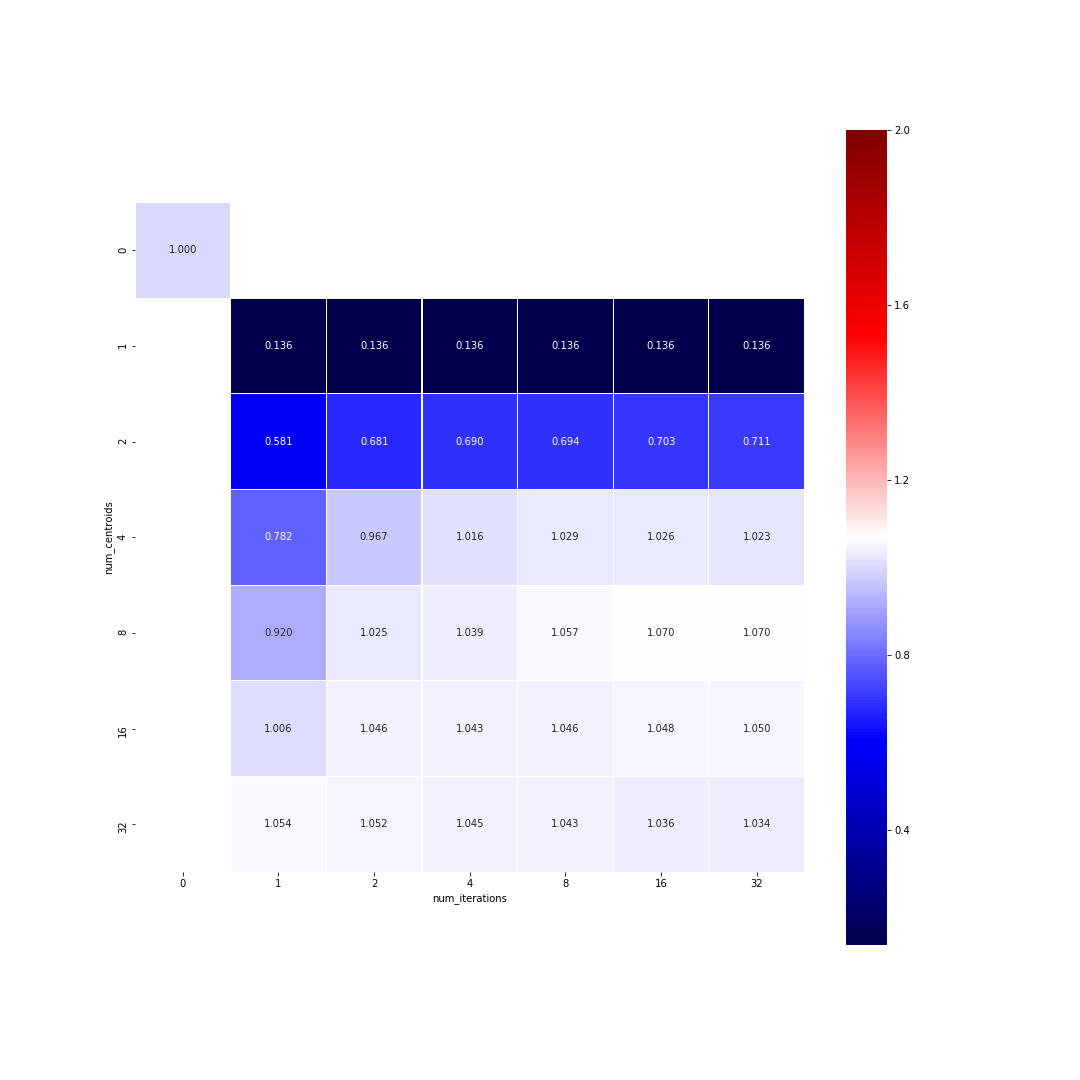
\includegraphics[width=0.9\textwidth]{photos/plots/jpg_vs_jpg}
    \caption{Wykres jakości wyników z tabeli \ref{m:jpg_vs_jpg}}
\end{figure}

Wprawdzie przy redukcji kolorów zdjęcia do jednego lub dwóch, daje to realną poprawę w porównaniu z rozmiarem oryginalnego zdjęcia. Widać jednak, że już przy czterech kolorach przestaje to powodować dużą różnicę w rozmiarze tak kompresowanych zdjęć.

\subsubsection{Porównanie formatów .jpg i .png}
\label{f:png_vs_jpg}

\begin{figure}[H]
	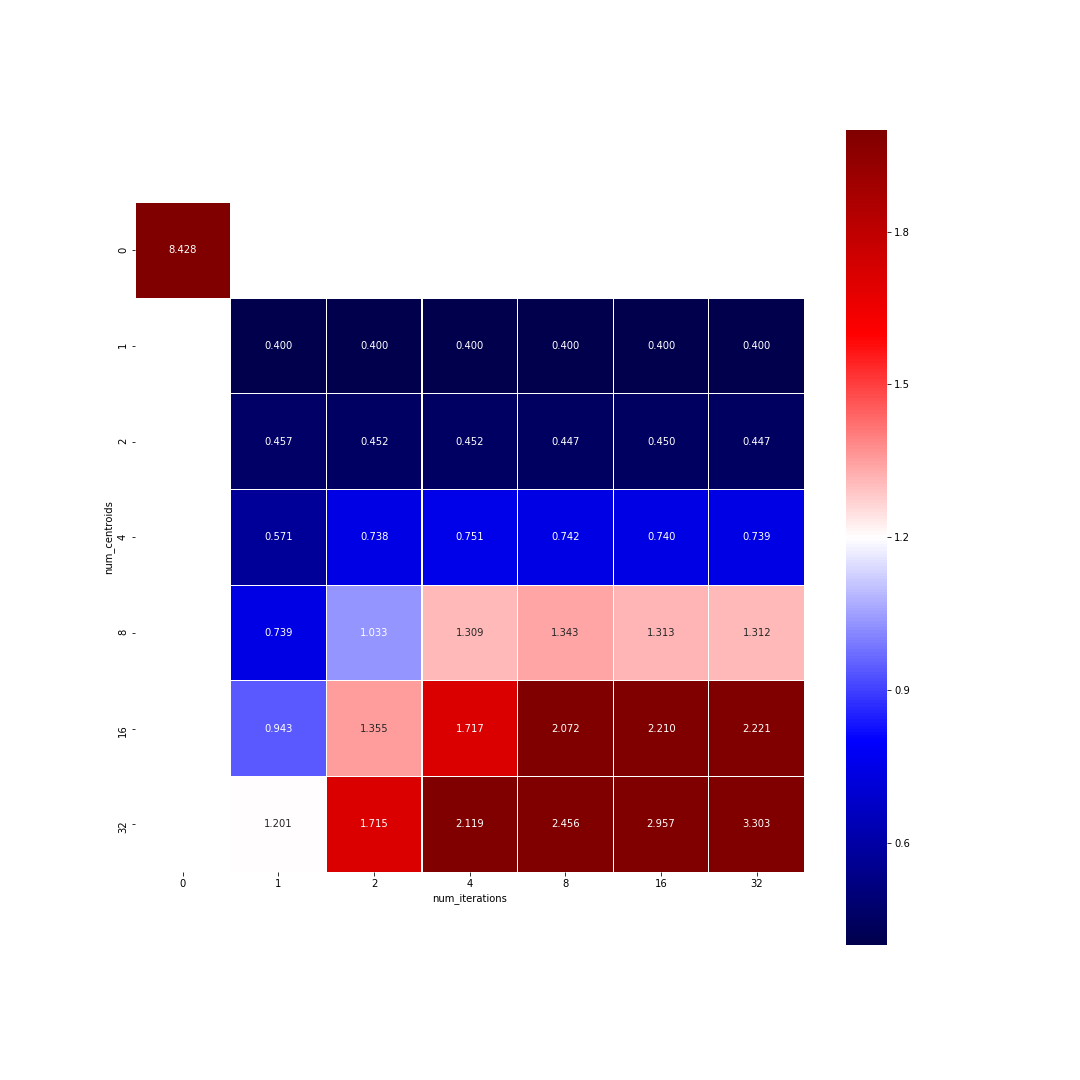
\includegraphics[width=0.9\textwidth]{photos/plots/png_vs_jpg}
    \caption{Wykres jakości wyników z tabeli \ref{m:png_vs_jpg}}
\end{figure}

Oryginalne zdjęcie zapisane w formacie .png jest ponad 8 razy większe niż to samo zdjęcie w formacie .jpg.
Choć sama redukcja kolorów obrazu (bez sprzętowej redukcji głębi obrazu) na początku działa na korzyść formatu .png. Jednak już przy redukcji do 8 kolorów widać, że na dłuższą metę nie jest ona wystarczająca, aby format .png dawał przewagę nad .jpg. Łącząc tę wiedzę z rezultatami z \ref{f:jpg_vs_jpg} można wysnuć wniosek, że ponieważ .png ze zredukowanymi kolorami nie daje przewagi nad .jpg z tak samo zredukowanymi kolorami, to nie będzie też dawać przewagi nad oryginalnym zdjęciem w formacie .jpg

\subsubsection{Porównanie formatu .png z redukcją głębi i bez}
\label{f:red_vs_png}

\begin{figure}[H]
	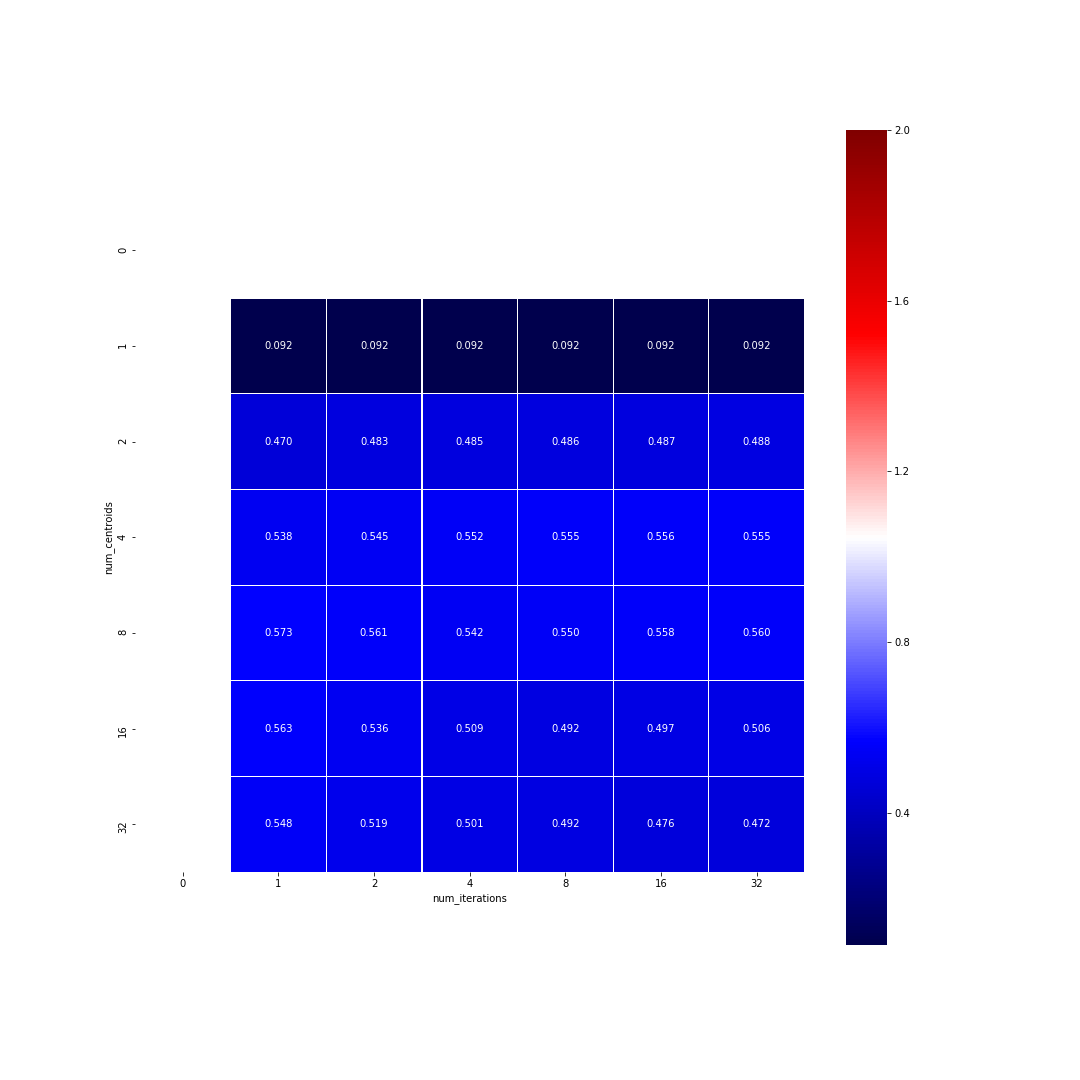
\includegraphics[width=0.9\textwidth]{photos/plots/red_vs_png}
    \caption{Wykres jakości wyników z tabeli \ref{m:red_vs_png}}
\end{figure}

Tutaj widać jednoznacznie, że użycie narzędzia systemowwego do redukcji głębi kolorów plików .png ze zdjęciami skutecznie obniża ich rozmiar ponad dwukrotnie. Co więcej, ponieważ oba zdjęcia mają uprzednio zredukowane kolory (za pomocą algorytmu k-means), redukcja głębi kolorów nie powoduje dalszych strat w jakości.

\begin{figure}[H]
  \centering
  \begin{minipage}[b]{0.4\textwidth}
    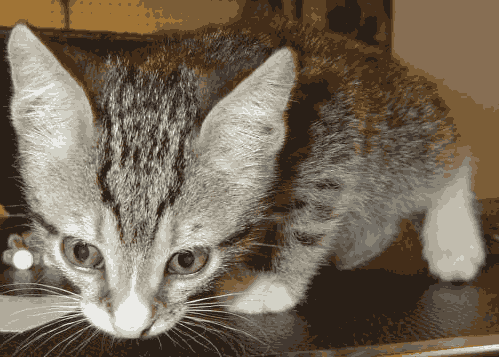
\includegraphics[width=\textwidth]{photos/kmeans_16_32}
    \caption{Zdjęcie zredukowane do 16 kolorów przed redukcją głębi kolorów pliku (91294 B)}
  \end{minipage}
  \hfill
  \begin{minipage}[b]{0.4\textwidth}
    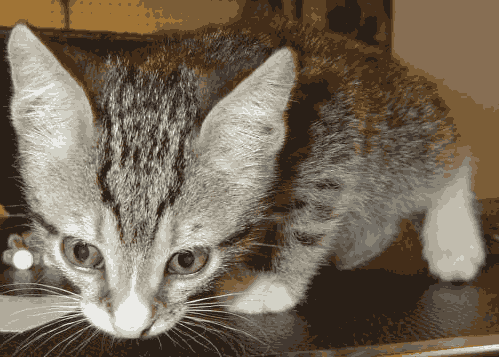
\includegraphics[width=\textwidth]{photos/kmeans_red_16_32}
    \caption{Zdjęcie zredukowane do 16 kolorów po redukcji głębi kolorów pliku (42138 B)}
  \end{minipage}
\end{figure}


\subsubsection{Porównanie rozmiaru doboru kolorów algorytmem k-means i systemowym w zdjęciach zdjęć w formacie .png z redukcją głębi kolorów}

\label{f:red_vs_red}

\begin{figure}[H]
	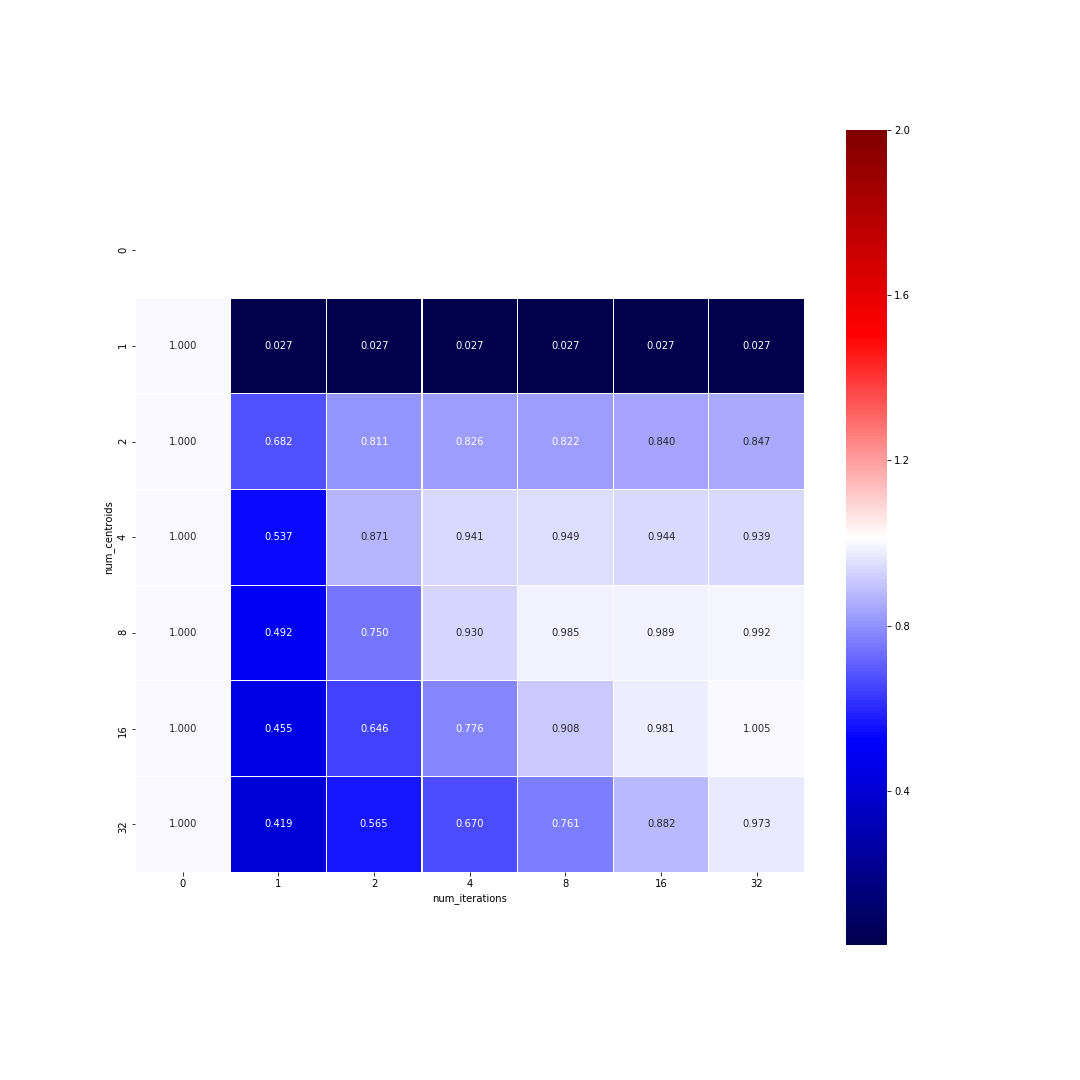
\includegraphics[width=0.9\textwidth]{photos/plots/red_vs_red}
    \caption{Wykres jakości wyników z tabeli \ref{m:red_vs_red}}
\end{figure}

Pierwsza kolumna ($num\_iterations = 0$) to rzecz jasna same wartości $1.0$, gdyż widać w niej porównanie średnich rozmiarów plików uzyskanych poprzez samą tylko systemową redukcję głębi kolorów (bez uprzedniej redukcji kolorów za pomocą k-means) z samymi sobą.

Dalsze kolumny przedstawiają ciekawsze wyniki, z których można wywnioskować, że dobór kolorów algorytmem k-means daje mniejszy lub porównywalny rozmiar zdjęć niż dobór kolorów poprzez narzędzie systemowe.

Co więcej, krótkie badania preferencyjne przeprowadzone na kilku osobach wykazały, że dobór kolorów uzyskiwany za pomocą k-means najczęściej milszy oku i bardziej przypominający oryginał.

\begin{figure}[H]
  \centering
  \begin{minipage}[b]{0.25\textwidth}
    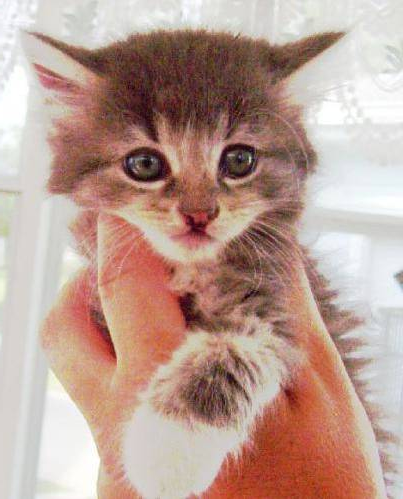
\includegraphics[width=\textwidth]{photos/original}
    \caption{Zdjęcie oryginalne (282801 B)\\\\\\\\}
  \end{minipage}
  \hfill
  \begin{minipage}[b]{0.25\textwidth}
    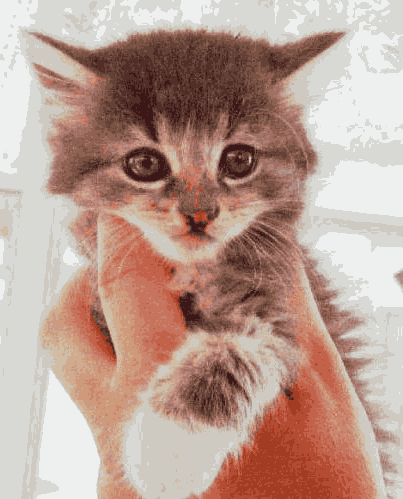
\includegraphics[width=\textwidth]{photos/kmeans_red_32_16}
    \caption{Zdjęcie zredukowane do 32 kolorów przez 16 iteracji k-means po redukcji głębi kolorów pliku (45795 B)}
  \end{minipage}
  \hfill
  \begin{minipage}[b]{0.25\textwidth}
    
\includegraphics[width=\textwidth]{photos/kmeans_red_32_0}
    \caption{Zdjęcie zredukowane do 32 kolorów wyłącznie poprzez redukcję głębi kolorów pliku (47415 B)}
  \end{minipage}
\end{figure}


\subsubsection{Porównanie obrazów w formacie .png ze zredukowaną głębią kolorów z oryginalnym zdjęciem w formacie .jpg}

\label{f:red_vs_jpg}

\begin{figure}[H]
	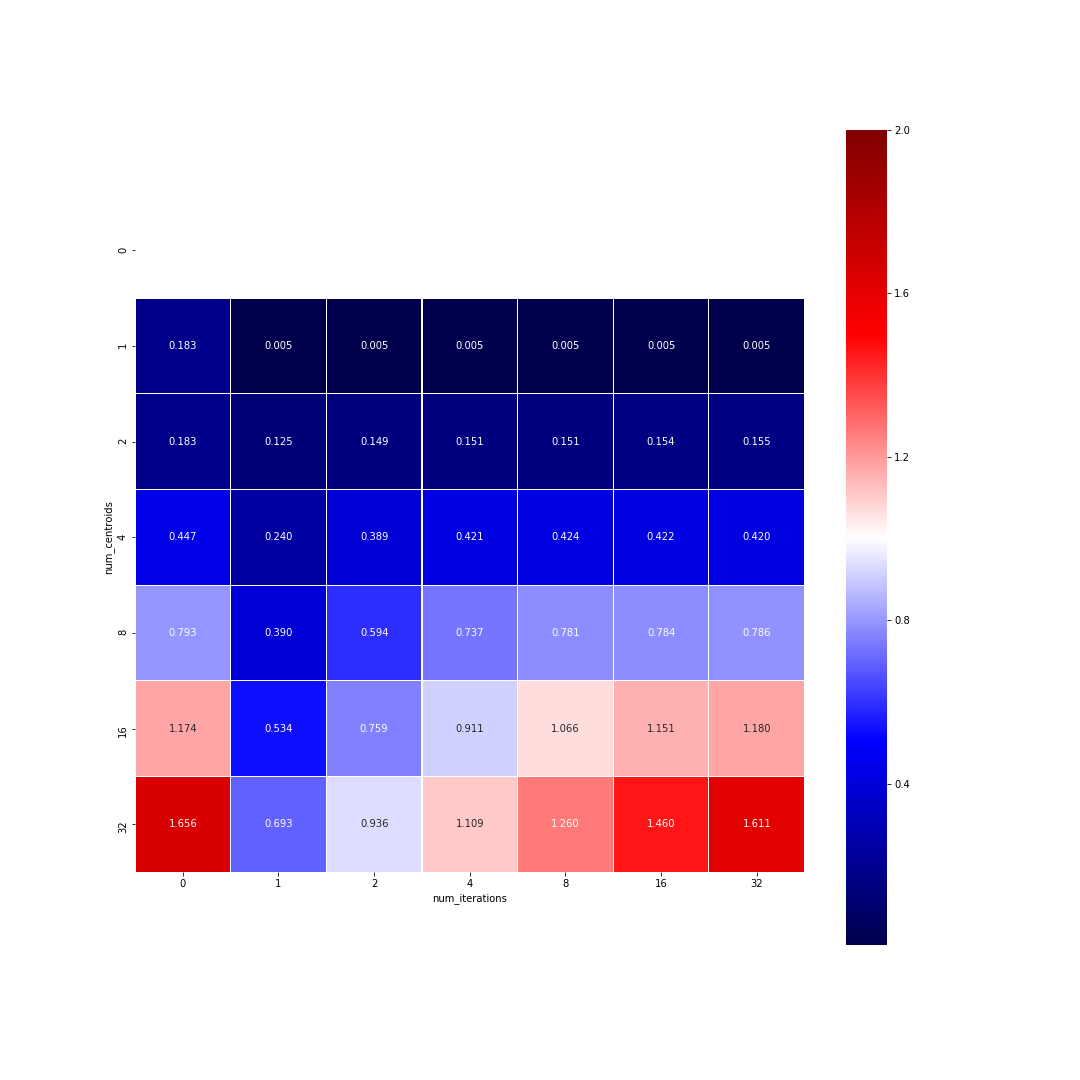
\includegraphics[width=0.9\textwidth]{photos/plots/red_vs_jpg}
    \caption{Wykres jakości wyników z tabeli \ref{m:red_vs_jpg}}
\end{figure}

Widać, że w większości przypadków skompresowane poprzez redukcję głębi obrazy .png mają mniejszy rozmiar niż oryginalny obraz zapisany jako .jpg. Niemniej jednak im lepsza jakość skompresowanego obrazu (więcej kolorów, więcej iteracji), tym bardziej porównanie wychodzi na korzyść oryginalnego .jpg.

\subsection{Wnioski dodatkowe}

Podczas pomiaróœ poczyniliśmy dodatkowe obserwacje:
\begin{enumerate}
\item Algorytm k-means (a przynajmniej nasza jego implementacja) działa dość powoli testowany na laptopie. Jego implementacja np. z biblioteki OpenCV będzie zapewne szybsza.
\item Narzędzie systemowe, choć daje nieco większe i nieco gorsze wizualnie obrazy, działa znacznie szybciej od naszej implementacji k-means.
\end{enumerate}

\section{Podsumowanie}

Podczas naszych badań udało nam się zaimplementować algorytm k-means, który z sukcesem redukuje liczbę kolorów w obrazie. Redukcja kolorów ma pozytywny wpływ na rozmiar obrazu, gdy zapisaujemy go w formacie .png - tego wpływu nie obserwujemy na dłuższą metę gdy zapisujemy obraz w formacie .jpg.

Sprawia to, że sama redukcja kolorów nie przynosi pożądanych skutków - format .jpg osiąga lepsze wyniki od .png rozszerzonego o redukcję.

Użytek ww. narzędzia systemowego, które fizycznie zmniejsza głębię kolorów w plikach .png znacznie poprawia wyniki kompresji. Przy odpowiednio niskiej liczbie kolorów, tak skompresowane pliki .png osiągają mniejsze rozmiary niż oryginalny .jpg oraz pliki .jpg skompresowane analogicznie.

Co więcej, zauważamy że selekcja odpowiednich kolorów za pomocą algorytmu k-means (zamiast kazać to robić narzędziu systemowemu) dodatkowo poprawia działanie narzędzia. Wynikowe obrazy są lepsze wizualnie przy mniejszym lub porównywalnym rozmiarze, co wyniki użycia samego tylko narzędzia.

Ostatecznie jednak udaje się nam uzyskać niższy rozmiar niż pliki .jpg tylko przy niskich liczbach kolorów (wyniki przestają być zadowalające przy 16), do których redukujemy obrazy. Należy sobie zadać pytanie, jaka jest dolna granica liczby kolorów do której redukujemy, przy której obraz wciąż będzie zadowalający wizualnie i nadający się do badania.

Choć nie badaliśmy tego formalnie, to zauważyliśmy że nasza implementacja k-means działa względnie powoli (rząd wielkości sekund), badana na laptopie z procesorem Intel Core i7. Można się tylko spodziewać, że działając na Raspberry Pi 1, czas takiej kompresji obrazów będzie o rzędzy wielkości dłuższy niż zaobserwowany dotychczas.

Rodzi to podejrzenie, czy używając k-means w celu zredukowania zużytej pamięci dyskowej faktycznie zdążymy w praktyce tę pamięć zapełnić. To podejrzenie w połączeniu z powyższymi obserwacjami skłania nas do wybrania w trakcie eksperymentu zapisu w formacie .jpg. Pomimo, że redukcja kolorów ma dobry wpływ na rozmiar obrazu, to w naszym konkretnym przypadku nie znajdujemy dla niej dużego zastosowania.
